\documentclass[aspectratio=169]{beamer}
\usetheme{metropolis}

\definecolor{main}{RGB}{92, 138, 168}
\definecolor{background}{RGB}{240, 247, 255}

\usepackage{booktabs}
\usepackage{amsmath}
\usepackage{amssymb}
\usepackage{amsfonts}
\usepackage{amsthm}
\usepackage{mathdots}
\usepackage{mathtools}
\usepackage{cancel}
\usepackage{braket}
\usepackage{listings}
\usepackage{ragged2e}

\newcommand{\git}{Git{}}
\newcommand{\cd}[1]{\texttt{#1}}

\apptocmd{\frame}{}{\justifying}{}

\title{\git, GitHub and GitFlow}
\author{Jacopo Schiavon}
\institute[Dep. Statistical Sciences --- UNIPD]{Department of Statistical Sciences\\ University of Padova}


\begin{document}
\begin{frame}[plain]
    \maketitle
\end{frame}

\begin{frame}{}
\tableofcontents
\end{frame}

\section{Introduction to \git}
\begin{frame}{What is \git?}
    \alert{\git} is a \alert{free} and \alert{open source} distributed \alert{version control system} (VCS) designed to handle everything from small to very large projects with speed and efficiency. 
    
    Its goals include \alert{speed}, \alert{data integrity}, and support for \alert{distributed} and \alert{non-linear} workflows.
    
    \begin{block}{History of \git}
        \begin{itemize}
        \justifying
            \item Created in 2005 by Linus Torvald (now maintained by Junio Hamano)
            \item Its original purpose was helping developing the Linux kernel
            \item It is designated for coordinating the work of many developer on the same project
            \item It is very useful also for smaller projects
        \end{itemize}
    \end{block}
    \note{This is a note}
\end{frame}

\begin{frame}{Why \git?}
    \git{} is used to manage projects consisting of \alert{text files}: \cd{R} or \cd{Python} packages and scripts; \LaTeX{} documents; repositories of text files (\textit{i.e.} configs for servers or desktops).
    
    Its most advanced features are useful when cooperating in a team of developers.
    \begin{block}{Why \git{} also for small project?}
        \begin{itemize}
        \justifying
            \item It teaches \alert{good practices} in developing and maintaining code
            \item It greatly simplify \alert{versioning} 
            \item It rationalize the management of new or experimental features
            \item Combined with GitHub, it trivialize \alert{code sharing}
            \item It helps with keeping track of the \alert{history of the code}.
        \end{itemize}
    \end{block}
\end{frame}

\begin{frame}{How \git{} works: basic concept}
    \git{} handles content in snapshots, one for each \alert{commit}, and knows how to apply or roll back the \alert{change sets} between two snapshots: for each new snapshot (commit), \git{} obtains the set of differences with the previous one.
    
    This is highlighted by the existence of the command \cd{git add}: in practice, when you are working in a directory three layer exists: 
    \begin{itemize}\justifying
        \item the \alert{previous commit} layer, with all the file as they were when you started
        \item the \alert{modified files} layer, with the files you are changing
        \item the \alert{staging area}, with files that you deem ready to commit
    \end{itemize}
    with the handy tool \cd{git diff} and its options you can always check the differences between files in the various layers and their previous state (or any point in history)
\end{frame}

\begin{frame}{\git{} features}
    \begin{itemize}
    \justifying
        \item \alert{Branching} \git{} main feature, will have an entirely dedicated slide.
        \item \alert{Small and Fast} All \git{} procedures (and \git{} itself) are fast and minimal: one or two commands to do everything. Committing and pushing requires no more than a couple of seconds $\Rightarrow$ almost no impact on the workflow.
        \item \alert{Entire history of the repository} \git{} keeps all versions of all files that it is tracking. Allows you to check differences between every two versions (or reverting to any version) of your code.
        \item \alert{Distribution} \git{} structure implies that each developer works on its own (\emph{forked}) version of a central repository, without breaking or interfering with the work of others developers.
        \item \alert{Cryptographic assurance} Every bit that \git{} tracks is authenticated by advanced cryptographic techniques.
    \end{itemize}
\end{frame}

\begin{frame}{\git{} features: Branching}
    \begin{itemize}
    \justifying
        \item Main idea: possibility to \alert{work in parallel} on the same code. 
        \item Useful also when working alone: possibility of \alert{testing different features} without creating copies. 
        \item A \alert{branch} is a new line of history of the code, completely independent from the rest
        \item \git{} allows to \alert{create}, \alert{switch} and \alert{merge} different branches with minimal effort (one command for each operation).
    \end{itemize}

    \begin{figure}
        \centering
        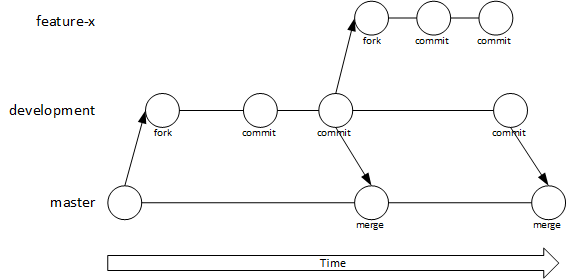
\includegraphics[height=0.4\textheight]{git_workflow_1.png}
    \end{figure}
\end{frame}

\begin{frame}{\git{} features: Branching}
    \begin{block}{Examples of use cases for small projects}
        \begin{itemize}
        \justifying
            \item Try a different implementation of a function not knowing if it will work better
            \item Try to rewrite a paragraph or chapter, not knowing if it will come out better
            \item Keep version of a document in another language
            \item Test a new functionality that might break another part of the code
        \end{itemize}
    \end{block}
\end{frame}

\begin{frame}{How to use it in practice? [UNIX systems]}
    UNIX systems are mainly MacOS or GNU/Linux (and others). Usually \git{} is \alert{already installed} in your system. If not, you can use your package manager on GNU/Linux (\emph{i. e.} \cd{apt install git} on Debian and derivatives), or the git installer from sourceforge\footnote{\url{http://sourceforge.net/projects/git-osx-installer/}} on MacOS
    \begin{block}{To create a \git{} repository:}
        \begin{itemize}
        \justifying
            \item Create the folder that you want to track with \git{} (or use one already in use)
            \item Open a terminal emulator and move to the location of the folder
            \item Give the magical command \cd{git init}
            \item You are ready to start committing!
        \end{itemize}
    \end{block}
\end{frame}

\begin{frame}{How to use it in practice? [Windows]}
    Usually \git{} is \alert{not installed} by default on Windows
    \begin{itemize}
    \justifying
        \item Download the windows installer from \url{https://git-scm.com/} and execute it.
        \item Follow the procedure for installation, installing the Git Bash.
        \item Now, clicking with the right button on a folder will allow you to open a Git Bash window, which will then allow you to work exactly as in a UNIX terminal (see previous slide).
    \end{itemize}
\end{frame}

\begin{frame}{How to use it in practice?}
    Once we have \git{} installed and a repository initiated, we start tracking the files in the folder that we are interested in by issuing the two command 
    \begin{flushleft}
        \cd{git add \textit{File1} \textit{File2} \textit{\dots}}\\
        \cd{git commit -m \textit{"First commit message"}}
    \end{flushleft}
    that tells \git{} to follow the files, then create the first commit. \git{} will now track every change to this files, and when we are satisfied with the changes we issue a new commit, \alert{snapshooting} a new point in the history of the file.
    
\end{frame}

\begin{frame}{How to use it in practice?}
    While we are working, it can be useful tu check the output of the two commands:
    \begin{flushleft}
        \cd{git status}\\
        \cd{git log --pretty=oneline}
    \end{flushleft}
    The first one gives you informations on the \alert{current status} of your repository: what file you modified since the last commit, if there are new untracked files in the folder and which files you added to the staging area. The second shows you the \alert{history of the project}, useful to obtain the commit name (a long alphanumeric code).
    
    Finally, the command \cd{git diff} helps to check \alert{changes} to files.
\end{frame}

\begin{frame}{How to use it in practice?}
    Sample output from various git commands:
    
    \begin{minipage}{0.32\textwidth}
        \cd{git status}
        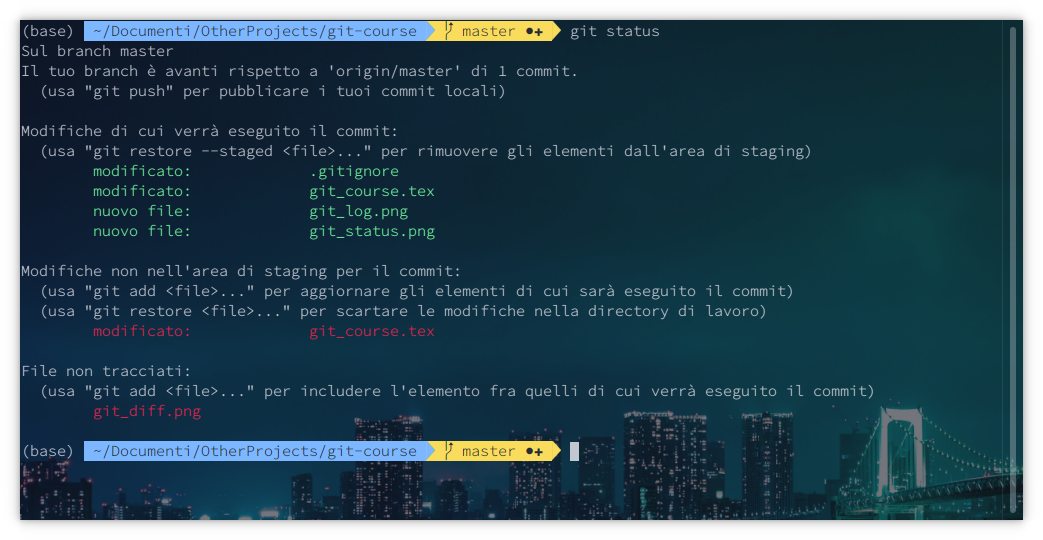
\includegraphics[width=\textwidth]{git_status.png}
    \end{minipage}
    \begin{minipage}{0.32\textwidth}
        \cd{git log}
        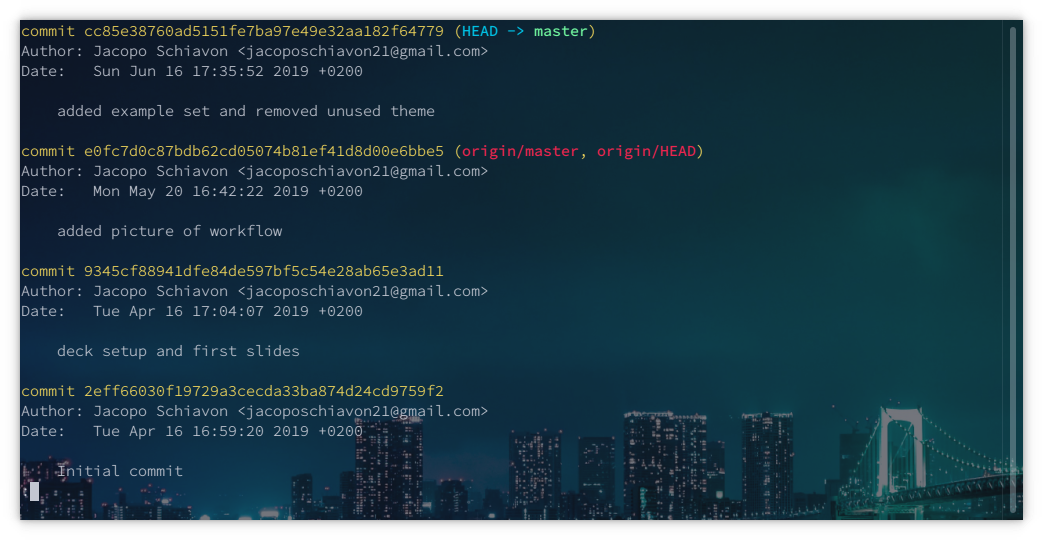
\includegraphics[width=\textwidth]{git_log.png}
    \end{minipage}
    \begin{minipage}{0.32\textwidth}
        \cd{git diff}
        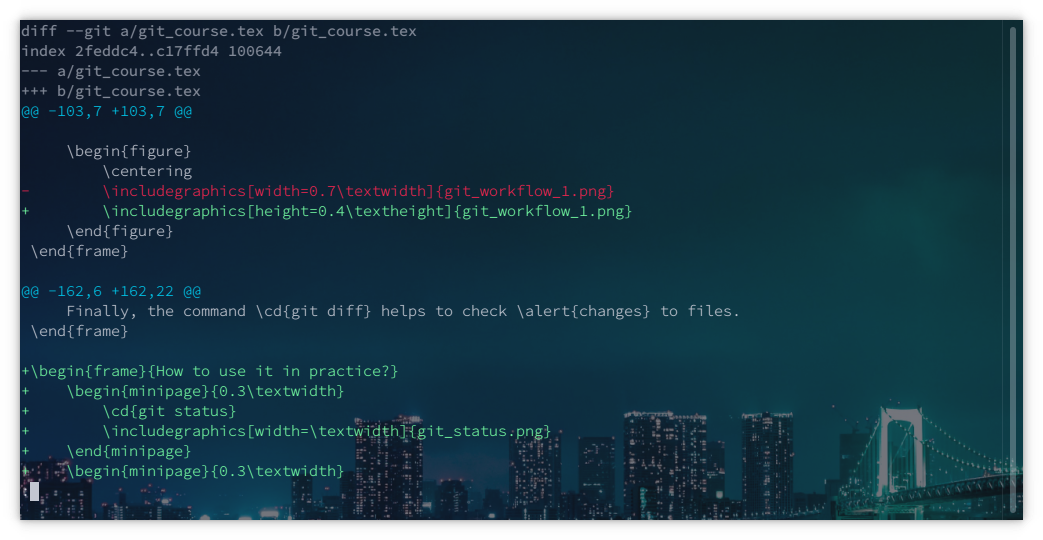
\includegraphics[width=\textwidth]{git_diff.png}
    \end{minipage}

    By creating a specific file named \cd{.gitignore} we can tell \git{} to \alert{ignore} specific files, subfolder or file format (we just need to list what we want to ignore). For instance, for a \LaTeX{} project we can ignore all the auxiliary files such as \cd{*.aux}, \cd{*.log}, \cd{*.out}\dots
\end{frame}



\section{Introduction to GitHub}
\begin{frame}{Why a remote repository?}
    \begin{itemize}
        \justifying
        \item The main idea behind \git{} is \alert{work parallelly} on the same project. This can be achieved only if the project (and thus the \git{} repository) is hosted online
        \item For a single developer, having a \alert{free remote version} of his project is very useful (for instance, to always have an backup of the code or to access it from everywhere)
        \item In this way it is easy to \alert{share the code}, to allow feedback from other developers and to adhere to EU compliances about open access
        \item Finally, this allows to easily \alert{distribute} our work (for instance an \cd{R} package).
    \end{itemize}
    There are many possible host for git repositories (GitLab, Bitbucket or SourceForge) but we will talk only of \alert{GitHub}, found at \url{https://www.github.com}
\end{frame}

\begin{frame}{GitHub: How it works}
    Actually, it is simply a matter of synchronizing the local repository with the online one.
    \begin{itemize}
        \justifying
        \item To start, one has to have a \alert{GitHub account}. Note that thank to the student pack\footnote{\url{https://education.github.com/pack}} you can have the pro version for free
        \item To create a \alert{new repository}, follow the simple instructions on the website
        \item If you want to obtain a local copy of the repository (that's the idea!) run a terminal (or a \git{} Bash) and type \cd{git clone} followed by the link to the repository (obtained from the green \alert{clone} button on GitHub)
    \end{itemize}
\end{frame}

%\section{Introduction to GitFlow}
%\begin{frame}{Frame Title}
%\end{frame}

\section{Some useful commands}
\begin{frame}{Local file management}
\begin{table}
    \scriptsize
    \centering
    \begin{tabular}{p{0.4\textwidth}p{0.5\textwidth}}
        \toprule
        \alert{Command}	&	\alert{Meaning}\\
        \midrule
        \cd{git init}	&	Initiate a local repository in the folder\\
        \cd{git status}	&	Shows the status of the file in the repository (new, modified, already stashed)\\
        \cd{git add [\textit{file}]}	&	Add \cd{\textit{file}} to the staging area\\
        \cd{git commit -m "\textit{msg}"} & Record a permanent snapshot of the staged files with an associated message \textit{msg}\\
        \cd{git log}	&	Shows the history of commits for the current branch\\
        \cd{git log -{}-pretty=oneline}	&	Shows a compressed version of the log\\
        \cd{git diff}	&	Shows not yet staged differences\\
        \bottomrule
    \end{tabular}
\end{table}
\end{frame}

\begin{frame}{Branching}
\begin{table}
    \scriptsize
    \centering
    \begin{tabular}{p{0.4\textwidth}p{0.5\textwidth}}
        \toprule
        \alert{Command}	&	\alert{Meaning}\\
        \midrule
        \cd{git branch}	&	List all branches\\
        \cd{git branch [\textit{name}]}	&	Create a branch named \textit{name}\\
        \cd{git checkout [\textit{name}]}	&	Switch to the branch named \textit{name}\\
        \cd{git merge [\textit{name}]}	&	Combines the branch named \textit{name} with the current branch\\
        \bottomrule
        \end{tabular}
    \end{table}
\end{frame}

\begin{frame}{Online repository}
\begin{table}
    \scriptsize
    \centering
    \begin{tabular}{p{0.4\textwidth}p{0.5\textwidth}}
        \toprule
        \alert{Command}	&	\alert{Meaning}\\
        \midrule
        \cd{git clone \textit{url}}	&	Download an online repository to your local filesystem\\
        \cd{git pull}	&	Download and integrate the online changes to the repository\\
        \cd{git fetch}	&	Download all the remote repository history\\
        \cd{git push [\textit{alias}] [\textit{branch}]}	& Pushes the local commits in the current branch to the \textit{branch} of online repository named \textit{alias}\\
        \bottomrule
        \end{tabular}
\end{table}
\end{frame}

\end{document}


